\documentclass[xcolor=table]{beamer}
\usepackage[utf8]{inputenc}
\usepackage[T1]{fontenc}
\usepackage[alf]{abntex2cite}
\usepackage{udesc}
\usepackage{amsfonts,amsmath,amssymb,mathtools}
\usepackage{verbatim}
\usepackage{listings}
\usepackage[ddmmyyyy]{datetime}
\usepackage{hyperref, url}
\usepackage{graphicx}
\usepackage{bussproofs}
\usepackage{multirow}
\usepackage{changepage}

\usepackage{svg}
\setsvg{inkscapeexe=inkscape}
\setsvg{inkscapeopt=-z -D}

\newcommand{\uglyphi}{\phi} % mantendo o \phi velho
\renewcommand \phi{\varphi}
\let \emptyset \varnothing

\newcommand{\Ltac}{$\mathcal{L}$\unskip tac}

\graphicspath{{Figuras/}}
\setbeamertemplate{frametitle continuation}{}

% suprimindo warnings do hyperref
\pdfstringdefDisableCommands{%
  \def\\{}%
  \def\texttt#1{<#1>}%
  \def\smallskip{}%
  \def\medskip{}%
}

\renewcommand{\figurename}{Figura}
\renewcommand{\tablename}{Tabela}
\sloppy
\title[]{Usando algoritmos determinísticos paralelos para escalonar tarefas em Edge-Cloud Continuum}

\author[Eliton Machado da Silva]{
    Eliton Machado da Silva\\\smallskip
    {\scriptsize Universidade do Estado de Santa Catarina \\\smallskip
    \vspace{-2mm}
    \texttt{eliton.mds@edu.udesc.br}\\\medskip
    {Orientador: Dr. Guilherme Piêgas Koslovski}\\
    }
}

\date{\today}

\begin{document}

    \begin{frame}
        \titlepage
    \end{frame}

    \begin{frame}[allowframebreaks]{Sumário}
        \tableofcontents
    \end{frame}

    \section[]{Introdução}
    
\begin{frame}{Introdução}
    \begin{columns}[T]
        \begin{column}{.5\textwidth}
            No mundo contemporâneo, dispositivos inteligentes e suas aplicações tornaram-se indispensáveis em nosso cotidiano.
            \begin{itemize}
                \item \textit{Cloud Computing}
            \end{itemize}
        \end{column}

        \begin{column}{.5\textwidth}
            \begin{figure}
                \centering
                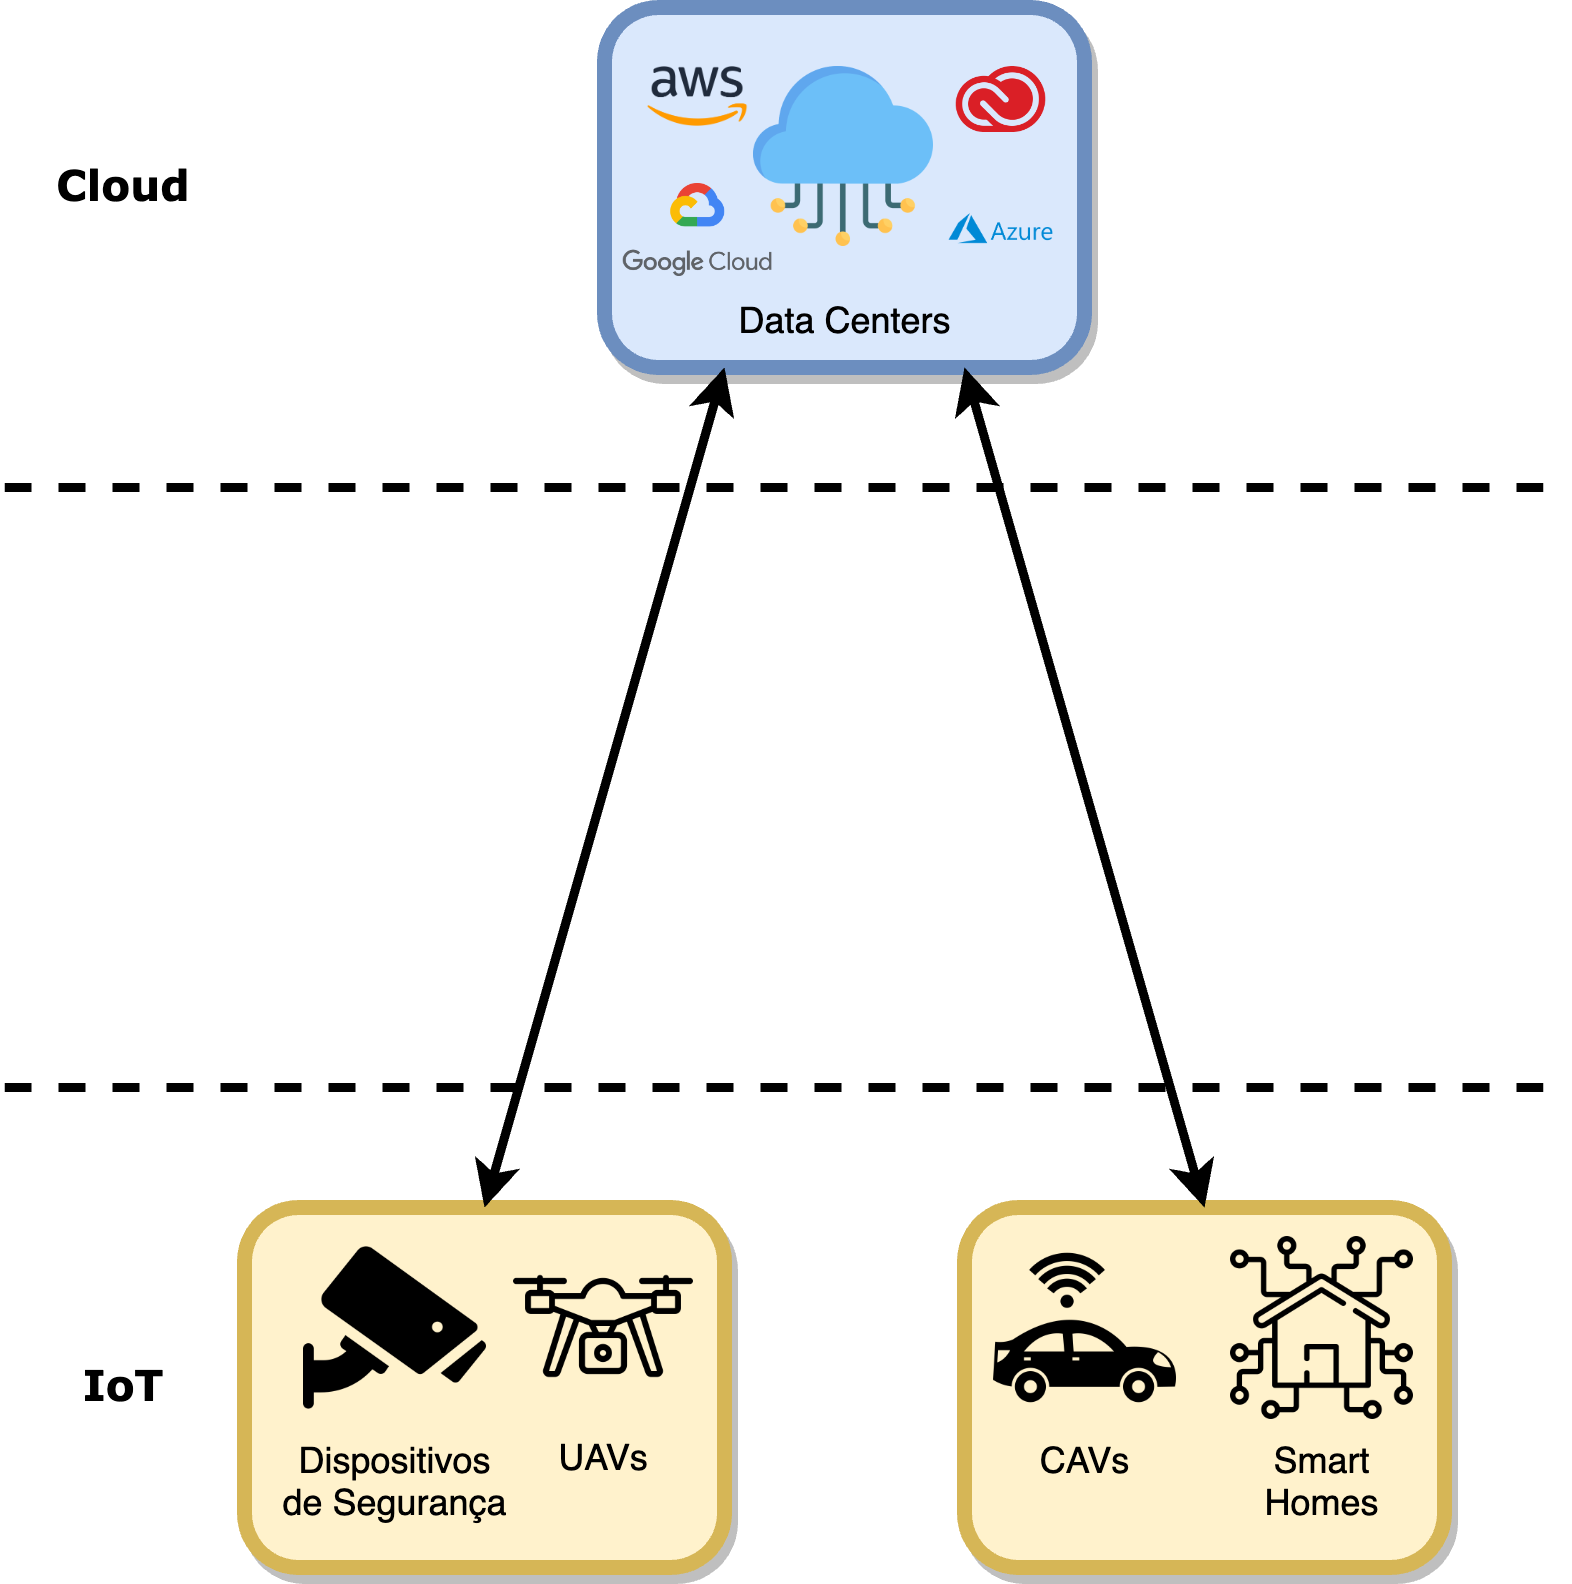
\includegraphics[width=\textwidth]{Figuras/TCC Cloud IoT.png}
            \end{figure}
        \end{column}
    \end{columns}
\end{frame}

\begin{frame}{Introdução}
    \begin{columns}[T]
        \begin{column}{.5\textwidth}
            Proposta inovadora que se concentra em oferecer capacidades de processamento nas proximidades do ponto de geração dos dados.
            \begin{itemize}
                \item \textit{Edge-Cloud Continuum}
                \begin{itemize}
                    \item[--] Escalonamento de recursos.
                \end{itemize}
            \end{itemize}
        \end{column}

        \begin{column}{.5\textwidth}
            \begin{figure}
                \centering
                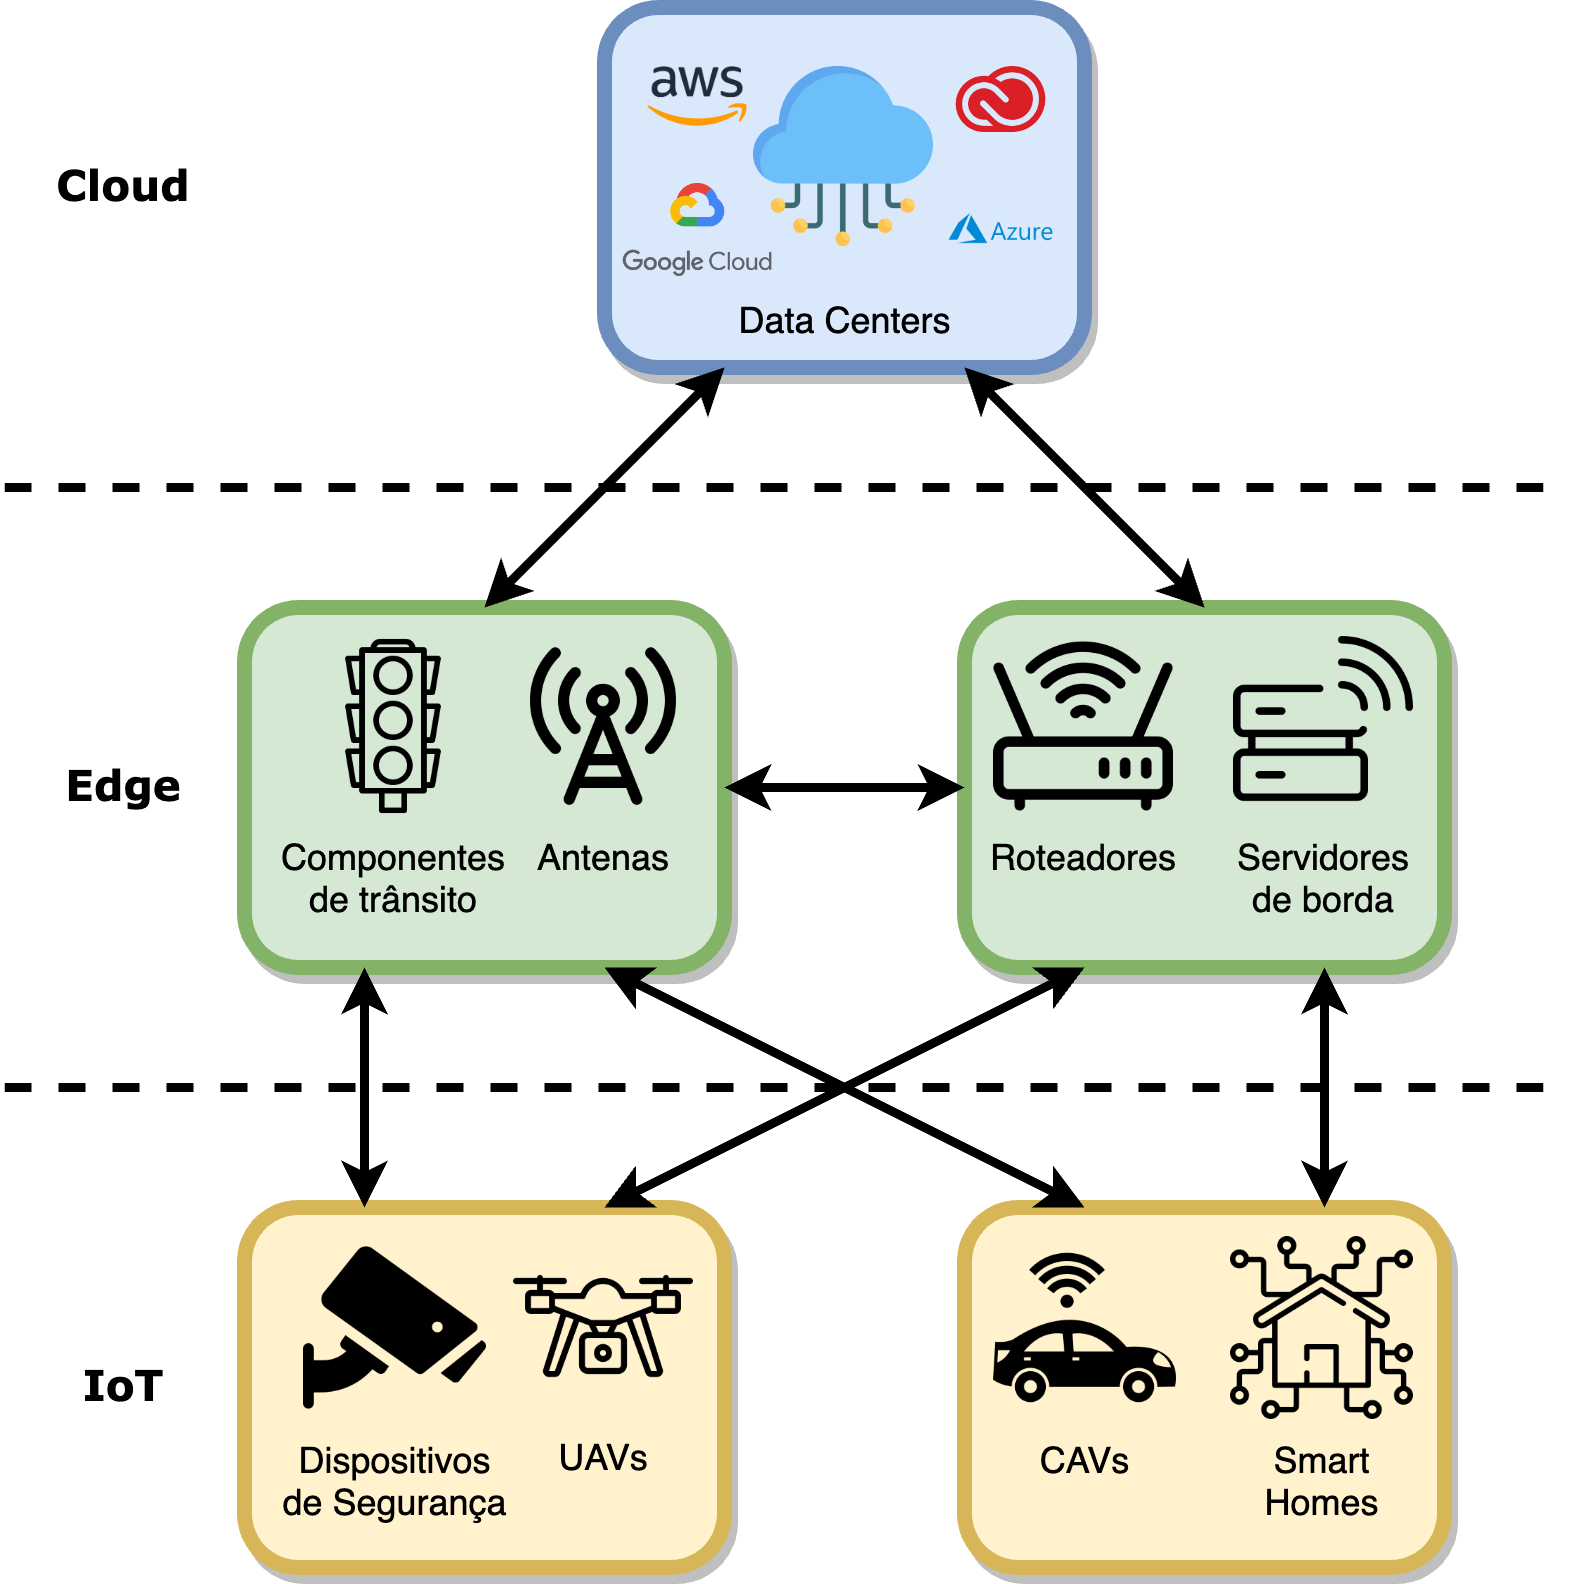
\includegraphics[width=\textwidth]{Figuras/TCC Edge Cloud IoT.png}
            \end{figure}
        \end{column}
    \end{columns}
\end{frame}

    \begin{frame}{Recursos}
    \begin{figure}
        \centering
        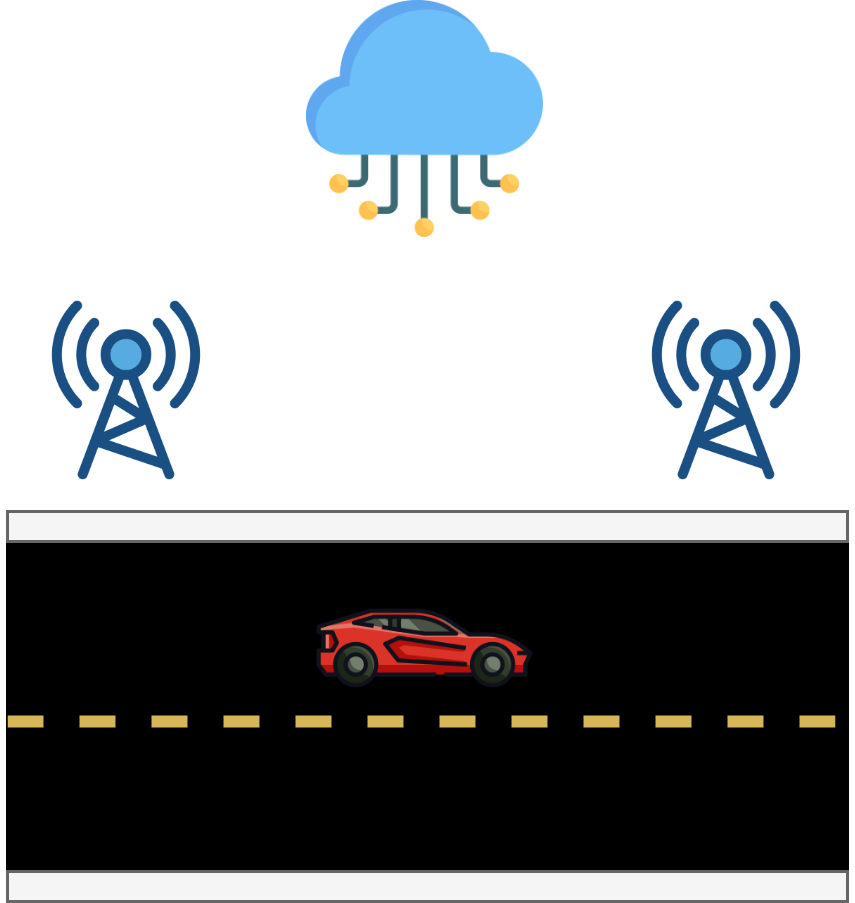
\includegraphics[width=0.7\textwidth]{Figuras/cav-scenario.png}
    \end{figure}
\end{frame}

\begin{frame}{Tarefas}
    \begin{figure}
        \centering
        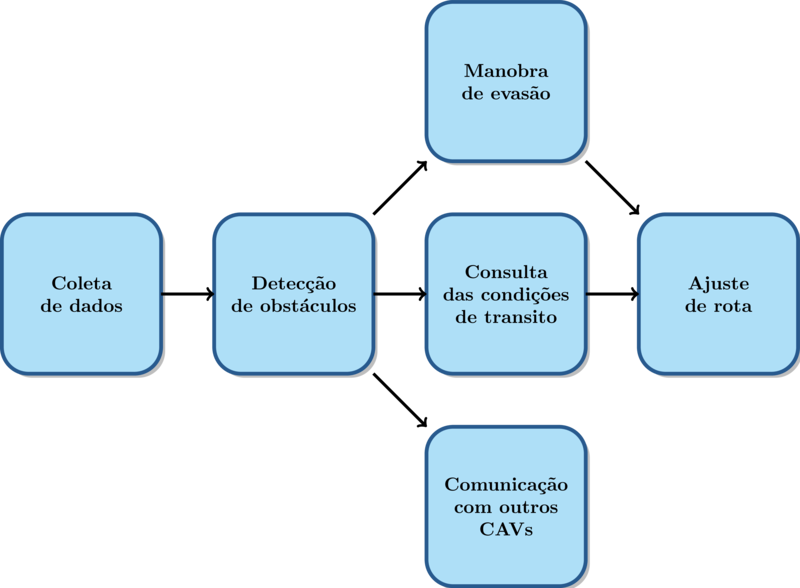
\includegraphics[width=0.8\textwidth]{Figuras/cav-task.png}
    \end{figure}
\end{frame}

\begin{frame}{Escalonamento}
    \begin{figure}
        \centering
        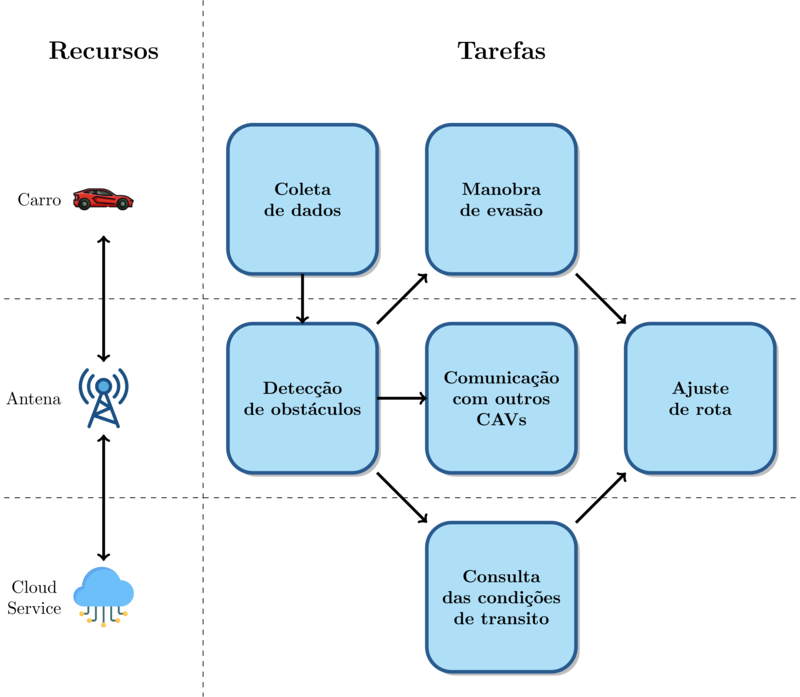
\includegraphics[width=0.8\textwidth]{Figuras/cav-scheduling.png}
    \end{figure}
\end{frame}

\begin{frame}{Escalonamento de Recursos}
    Problema conhecido na literatura.
    \begin{itemize}
        \item NP-Hard.
        \item Diversidade de soluções propostas.
        \begin{itemize}
            \item[--] ADMM, Heft, Page Rank, Polaris, etc.
        \end{itemize}
    \end{itemize}
\end{frame}

\begin{frame}{Escalonamento de Recursos}
    Dificuldades encontradas ao desenvolver algoritmos de escalonamento em Edge-Cloud Continuum:
    \begin{itemize}
        \item Modelagem do problema não padronizada.
        \item Código fechado.
        \item Falta de componentes comuns de alto desempenho.
    \end{itemize}
\end{frame}

\begin{frame}{Escalonamento de Recursos}
    Solução:

    Framework
    \begin{itemize}
        \item[] de código aberto
        \item[] que incorpora componentes comuns a algoritmos de escalonamento
        \item[] focado em alto desempenho.
    \end{itemize}
\end{frame}

    \section[]{Objetivos}
    \begin{frame}{Objetivos}
    Desenvolver um framework baseado em arquiteturas paralelas para
    escalonamento de tarefas em Edge-Cloud Continuum (ECC).
    \vspace{10px}
    \begin{enumerate}
        \item Estudar escalonamento em Edge-Cloud Continuum (ECC).
        \item Estudar as particularidades de arquiteturas paralelas.
        \item Estudar algoritmos determinísticos para escalonamento.
        \item Elaboração de um \textit{framework} inovador utilizando algoritmos determinísticos e arquiteturas paralelas para o problema de escalonamento de recursos.
        \item Implementação do \textit{framework} proposto.
        \item Análise da eficácia do \textit{framework} definido.
    \end{enumerate}
\end{frame}


    \section[]{Modelagem do problema}
    
\begin{frame}{Modelagem - Recursos}
    \begin{columns}[T]
        \begin{column}{.5\textwidth}
            Recursos:
            \begin{itemize}
                \item Infraestrutura da rede.
                \item Comunicação entre recursos.
                \item Grafo.
            \end{itemize}
        \end{column}

        \begin{column}{.5\textwidth}
            \begin{figure}
                \centering
                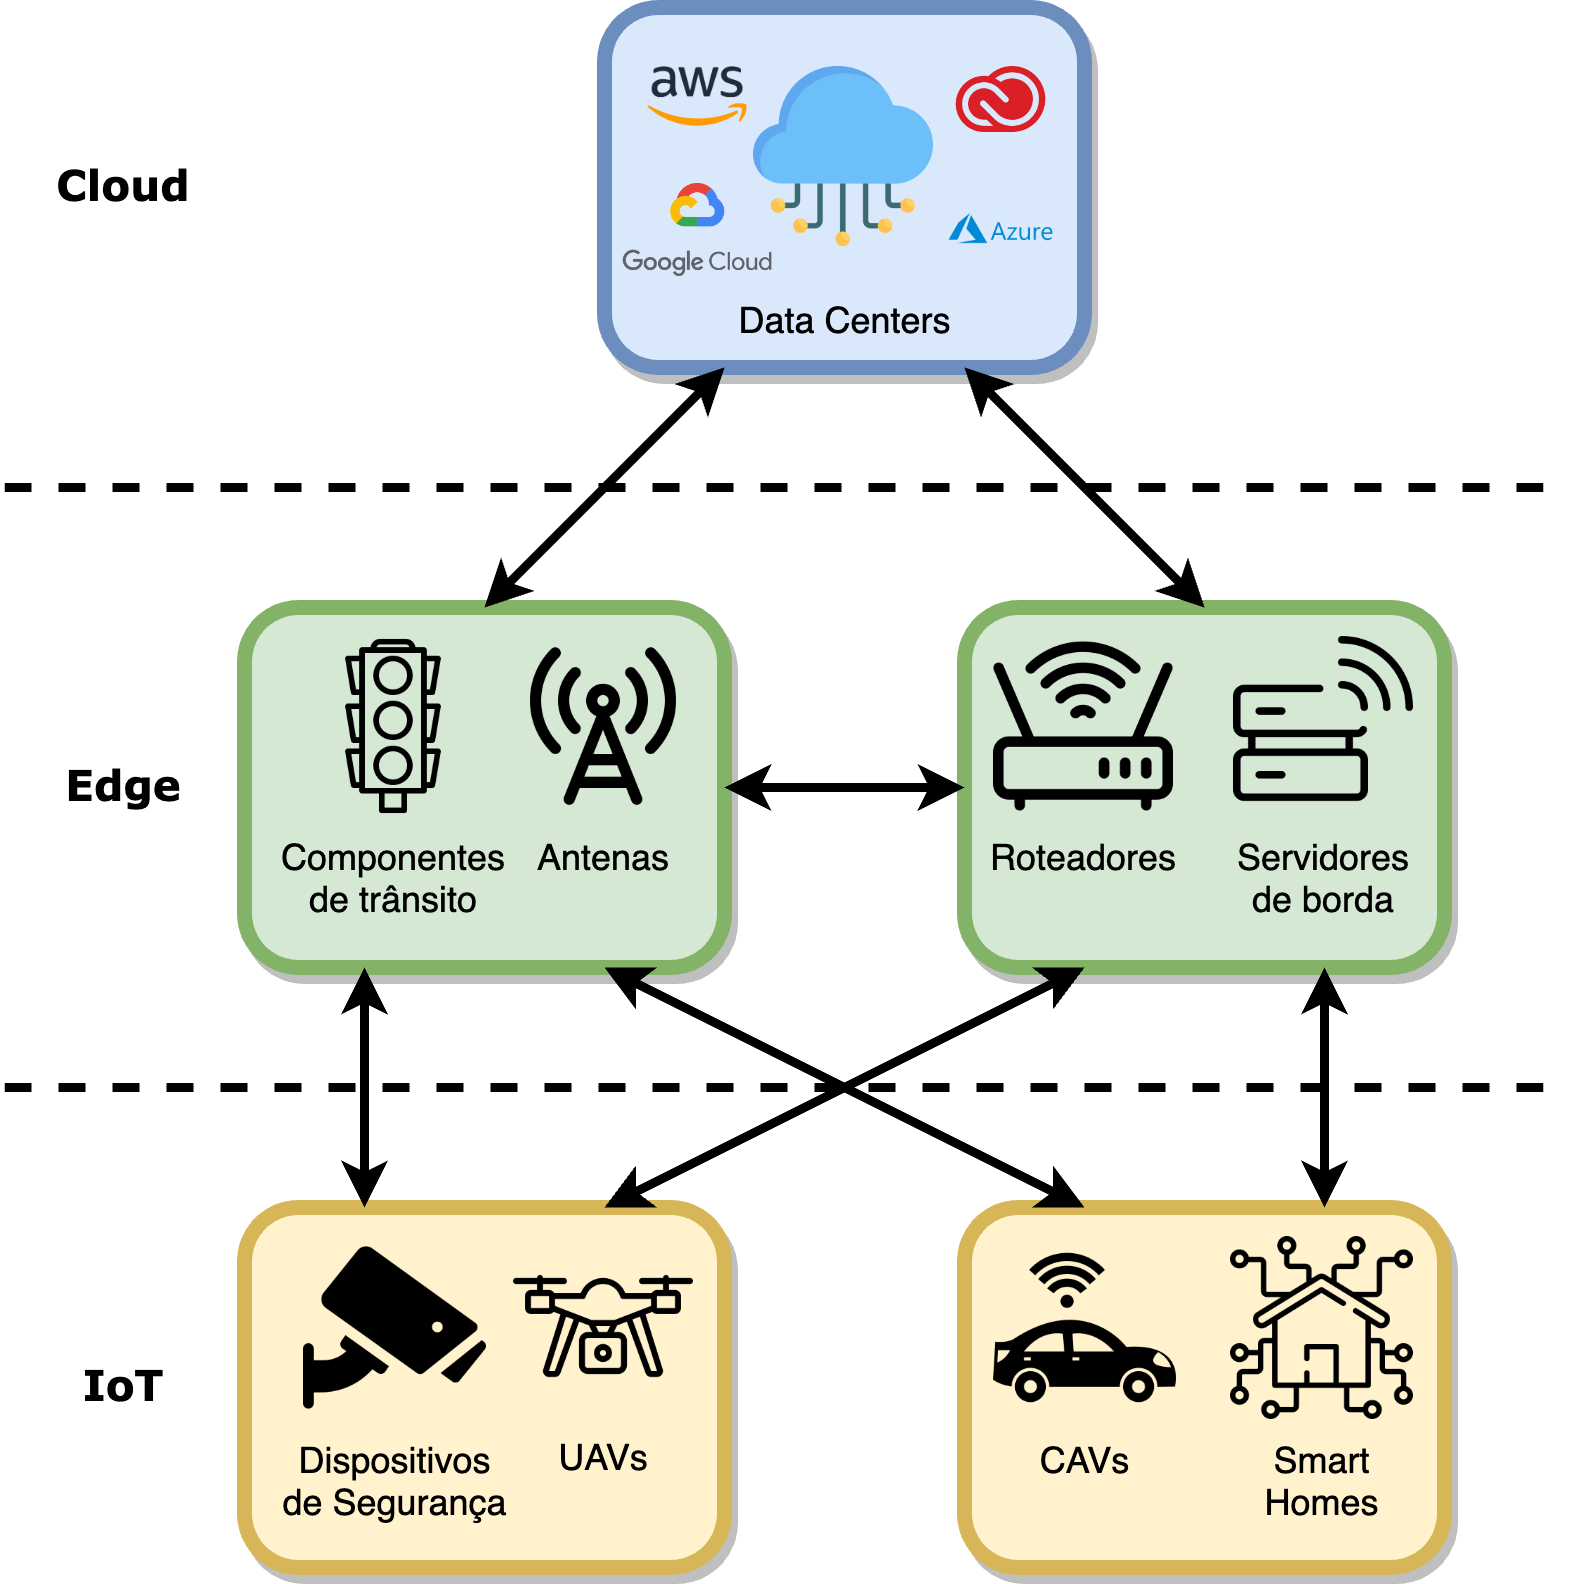
\includegraphics[width=\textwidth]{Figuras/TCC Edge Cloud IoT.png}
            \end{figure}
        \end{column}
    \end{columns}
\end{frame}

\begin{frame}{Modelagem - Tarefas}
    \begin{columns}[T]
        \begin{column}{.5\textwidth}
            Tarefas:
            \begin{itemize}
                \item Dados.
                \item Dependências de tarefas.
                \item Grafo acíclico e direcionado.
            \end{itemize}
        \end{column}

        \begin{column}{.5\textwidth}
            \begin{figure}
                \centering
                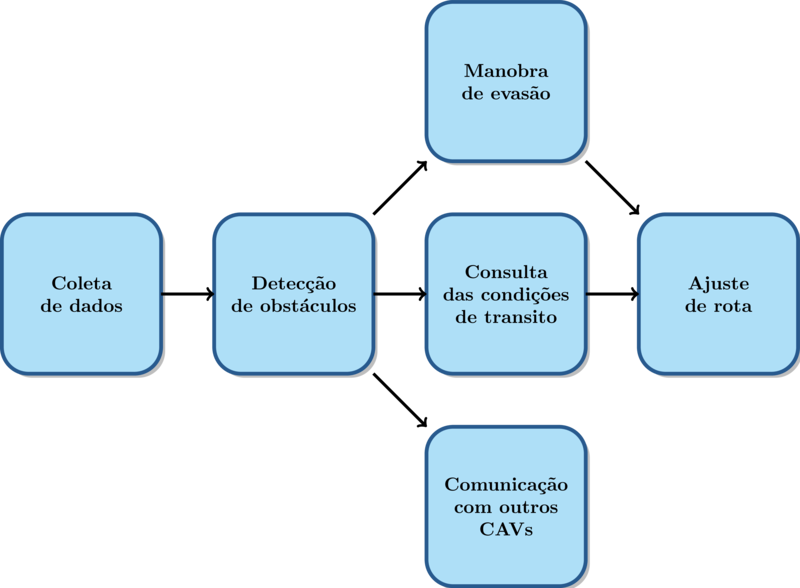
\includegraphics[width=\textwidth]{Figuras/cav-task.png}
            \end{figure}
        \end{column}
    \end{columns}
\end{frame}

\begin{frame}{Modelagem - Escalonamento}
    Escalonamento:
    \begin{itemize}
        \item Atribuir tarefas a recursos.
        \item Entrada:
        \begin{itemize}
            \item[--] Grafo de recursos.
            \item[--] DAG de tarefas.
        \end{itemize}
        \item Saída:
        \begin{itemize}
            \item[--] Sequencia de mapeamentos de tarefas para recursos.
        \end{itemize}
        \item Otimizar Política de escalonamento:
        \begin{itemize}
            \item[--] Minimizar tempo de processamento.
            \item[--] Minimizar consumo de energia.
        \end{itemize}
    \end{itemize}
\end{frame}

    % \section[]{Algoritmos determinísticos}
    % \section[]{Arquiteturas Paralelas}
    \section[]{Trabalhos Relacionados}

    \section[]{Framework Proposto}
    \begin{frame}{Proposta}
    \begin{enumerate}
        \item Trabalhos relacionados.
        \item Algoritmos.
        \begin{itemize}
            \item Algoritmos Determinísticos.
            \item Arquiteturas Paralelas.
        \end{itemize}
        \item Cenário de execução.
        \item Técnicas e ferramentas.
        \item Cenário de teste.
    \end{enumerate}
\end{frame}

\begin{frame}{Algoritmos Determinísticos}
    Algoritmos Determinísticos:

    \begin{itemize}
        \item Resultados consistentes para determinada entrada.
        \item Previsíveis.
        \item Garantia de solução ótima.
        \item Características essenciais para garantir confiabilidade no sistema.
    \end{itemize}
\end{frame}

\begin{frame}{Arquiteturas Paralelas}
    Arquiteturas Paralelas:

    \begin{itemize}
        \item \textit{SIMD} e \textit{MIMD}.
        \item Otimizar a execução de operações em grandes volumes de dados.
        \item Alto desempenho.
    \end{itemize}
\end{frame}

\begin{frame}{Trabalhos Relacionados}
    \begin{figure}
        \centering
        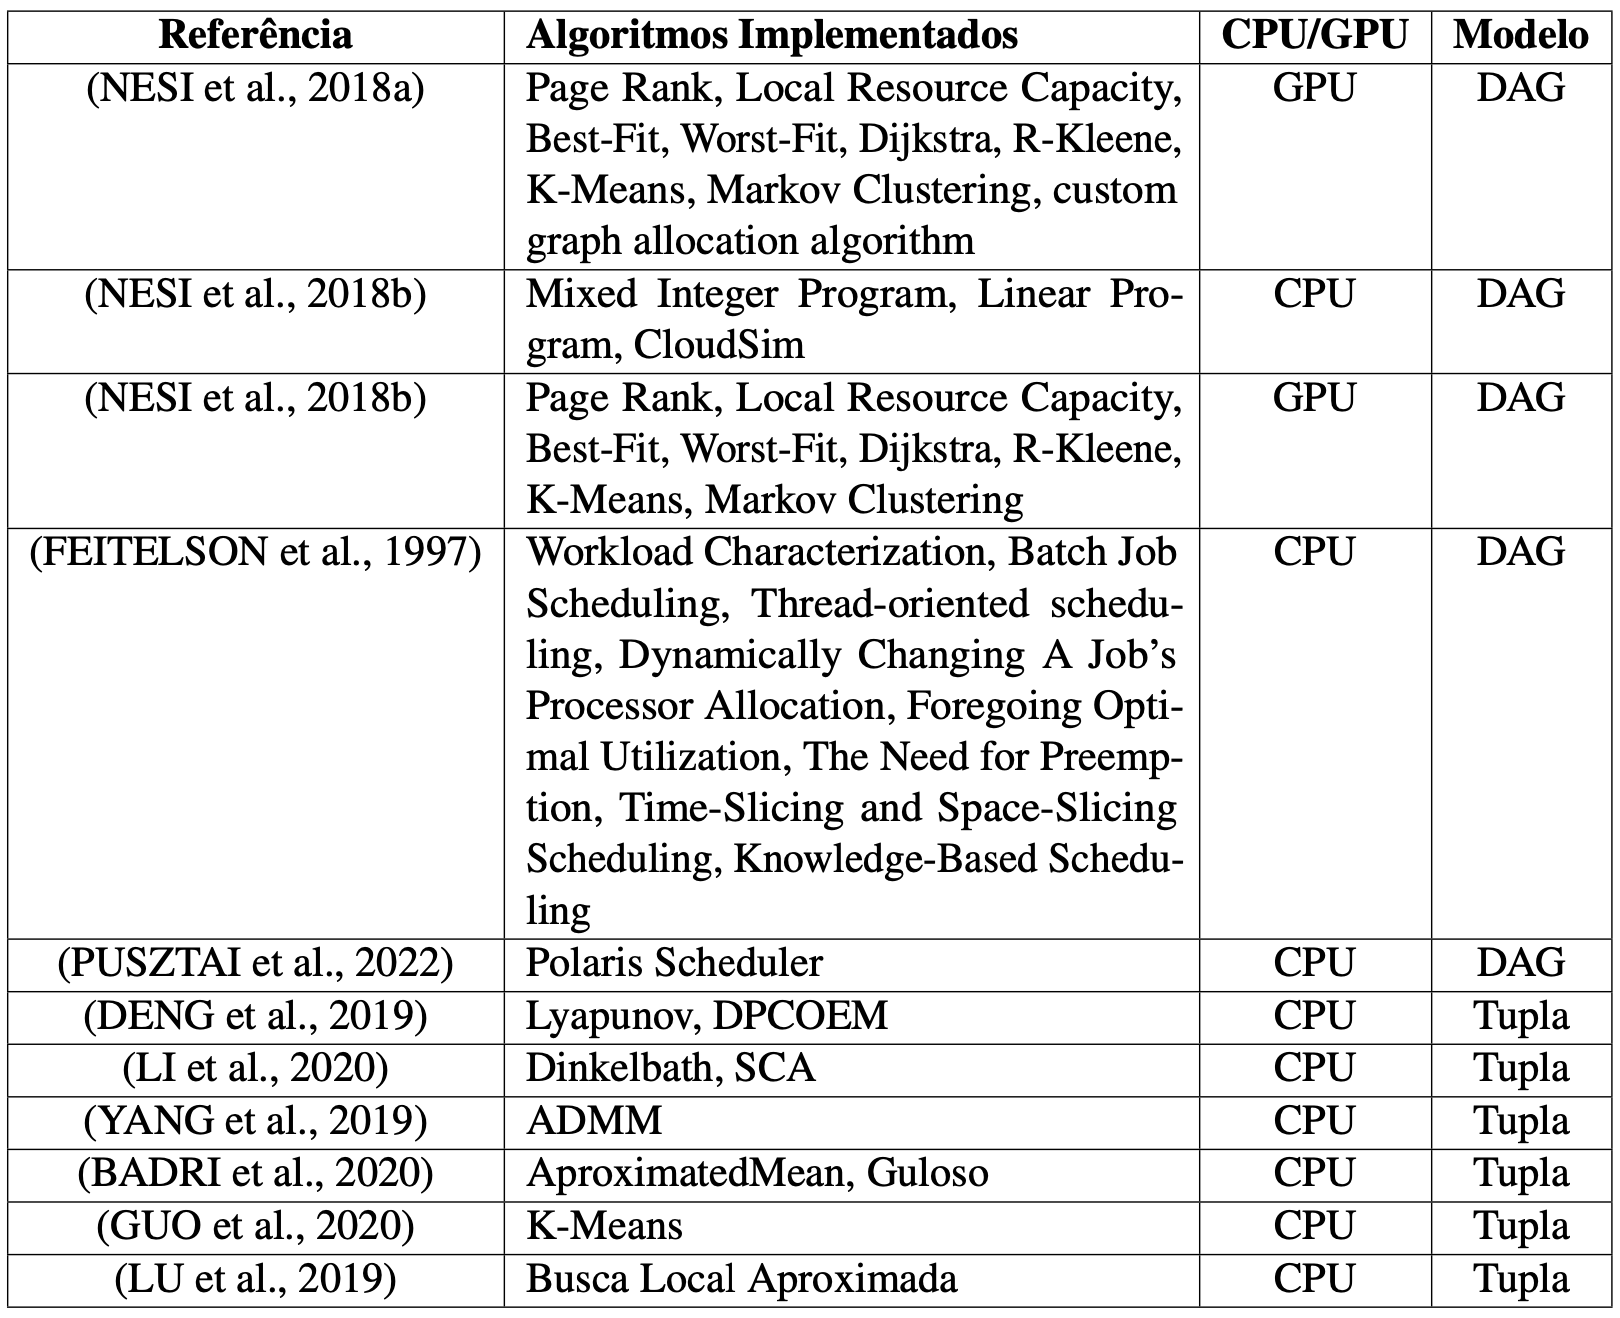
\includegraphics[width=0.9\textwidth]{Figuras/trabalhos-relacionados.png}
    \end{figure}
\end{frame}

\begin{frame}{Algoritmos}
    \begin{table}[ht]
        \centering
        \scriptsize
        \begin{tabular}{|c|c|c|c|}
            \hline
            \textbf{Algoritmo} & \textbf{Categoria} & \textbf{Complexidade} & \textbf{CPU/GPU} \\
            \hline
            Busca Binária & Busca & $O(\log n)$ & CPU \\
            \hline
            Merge Sort & Ordenação & $O(n \log n)$ & CPU \\
            \hline
            Topological Sort & Ordenação & $O(V + E)$ & CPU \\
            \hline
            Radix Sort & Ordenação & $O(nw)$ & GPU \\
            \hline
            K-means & Agrupamento & $O(nkdi)$ & GPU \\
            \hline
            DBSCAN & Agrupamento & $O(n^2)$ & GPU \\
            \hline
            Hierarchical Clustering & Agrupamento & $O(n^3)$ & CPU \\
            \hline
            Markov Clustering & Agrupamento & $O(n^3)$ & GPU \\
            \hline
            PageRank & Ranqueamento & $O(n + m)$ & GPU \\
            \hline
            Dijkstra & Menor Caminho & $O(E + V \log V)$ & CPU \\
            \hline
            Floyd-Warshall & Menor Caminho & $O(n^3)$ & CPU \\
            \hline
            A* & Menor Caminho & $O(E \log V)$ & CPU \\
            \hline
            Kruskal & MST & $O(E \log E)$ & CPU \\
            \hline
            Prim & MST & $O(E + V \log V)$ & CPU \\
            \hline
            Edmonds-Karp & Fluxo & $O(VE^2)$ & CPU \\
            \hline
            Min-Cost Max-Flow & Fluxo & $O(V^2E^2)$ & CPU \\
            \hline
            Dinic & Fluxo & $O(V^2E)$ & CPU \\
            \hline
            Gaussian Elimination & Otimização & $O(n^3)$ & GPU \\
            \hline
            Hungarian & Otimização & $O(n^3)$ & CPU \\
            \hline
            ADMM & Otimização & - & GPU \\
            \hline
        \end{tabular}
        \caption{Algoritmos presentes no \textit{framework} proposto.}
        \label{table:algorithms}
    \end{table}
\end{frame}

    
% talvez remover esse slide
\begin{frame}{Cenário de execução}
    \begin{figure}
        \centering
        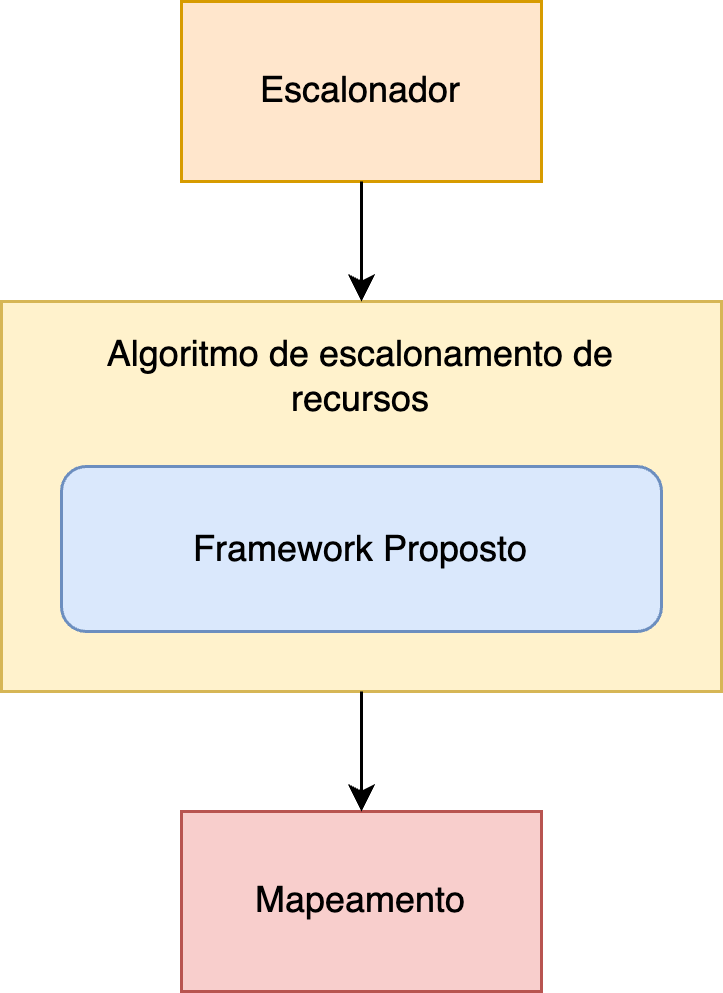
\includegraphics[width=0.5\textwidth]{Figuras/framework_usage.png}
    \end{figure}
\end{frame}

\begin{frame}{Código Exemplo}
    \begin{figure}
        \centering
        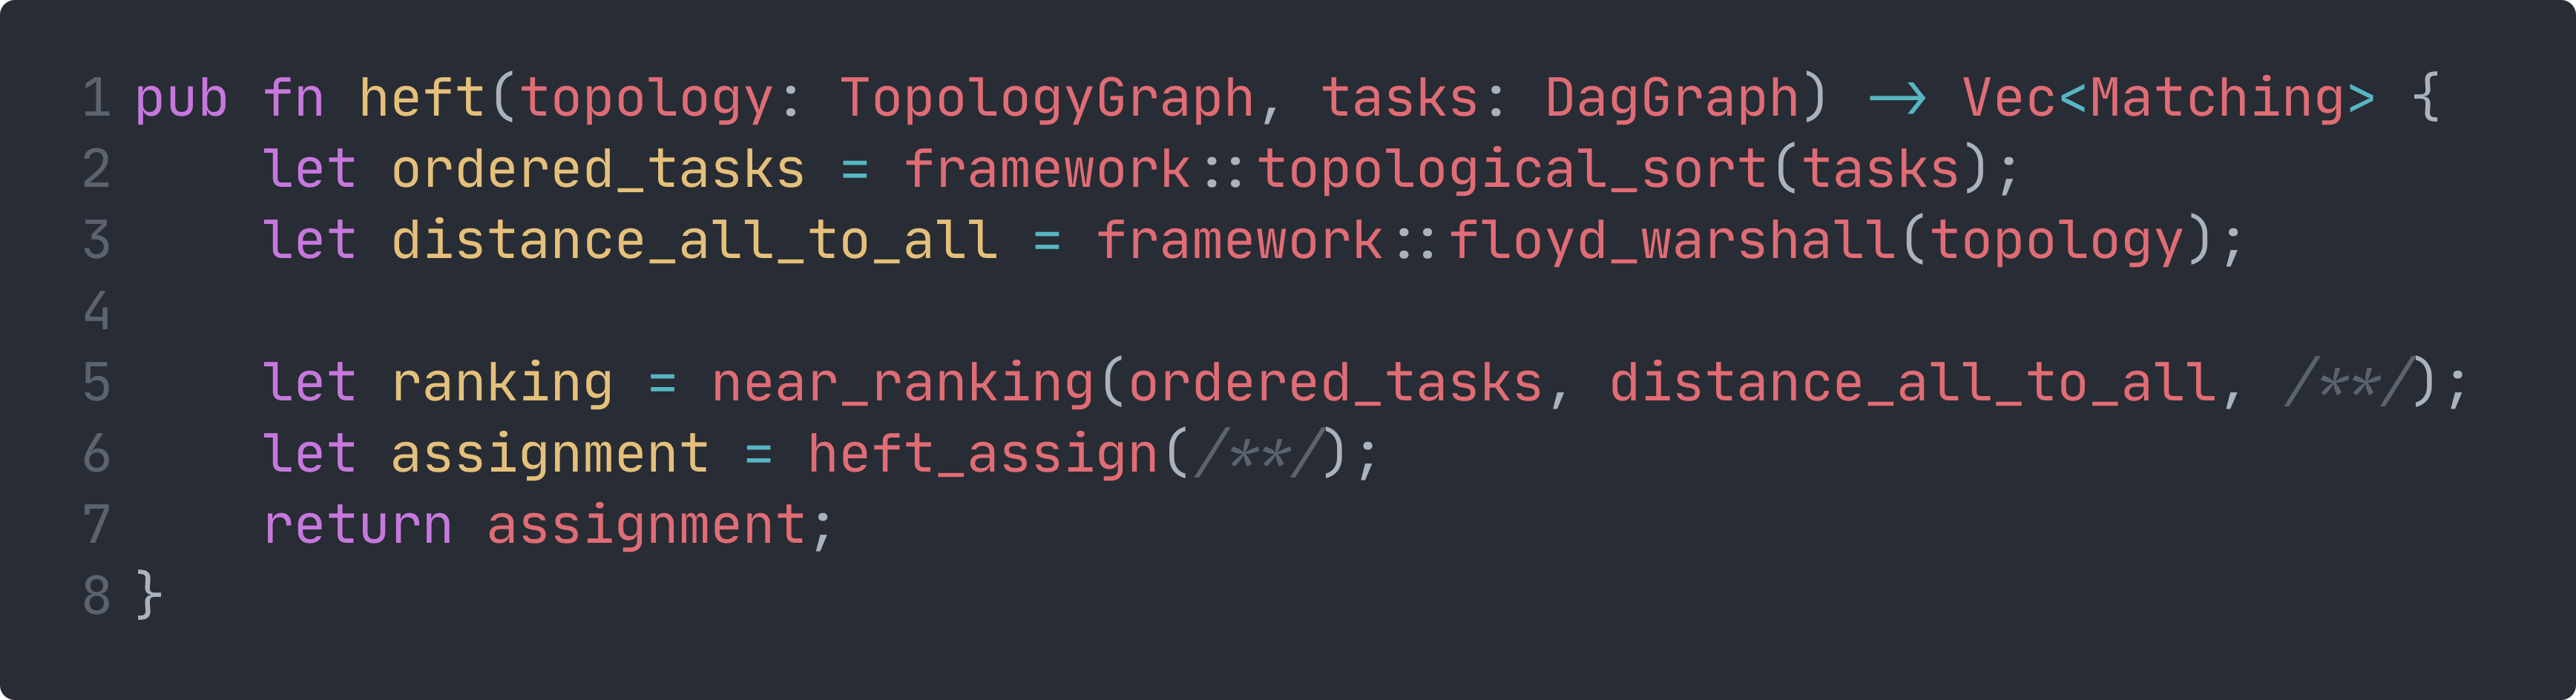
\includegraphics[width=\textwidth]{Figuras/code.png}
    \end{figure}
\end{frame}

\begin{frame}{Técnicas e Ferramentas}
    \begin{columns}
    \begin{column}{0.9\textwidth}
    Rust:
    \begin{itemize}
        \item[--] Linguagem moderna.
        \item[--] Segurança de memória.
        \item[--] Alto desempenho. 
        \item[--] \textit{Petgraph}.
        \item[--] \textit{Fearless Concurrency}.
        \item[--] \textit{Rayon}.
    \end{itemize}
    \end{column}

    \begin{column}{0.1\textwidth}
        \begin{figure}
            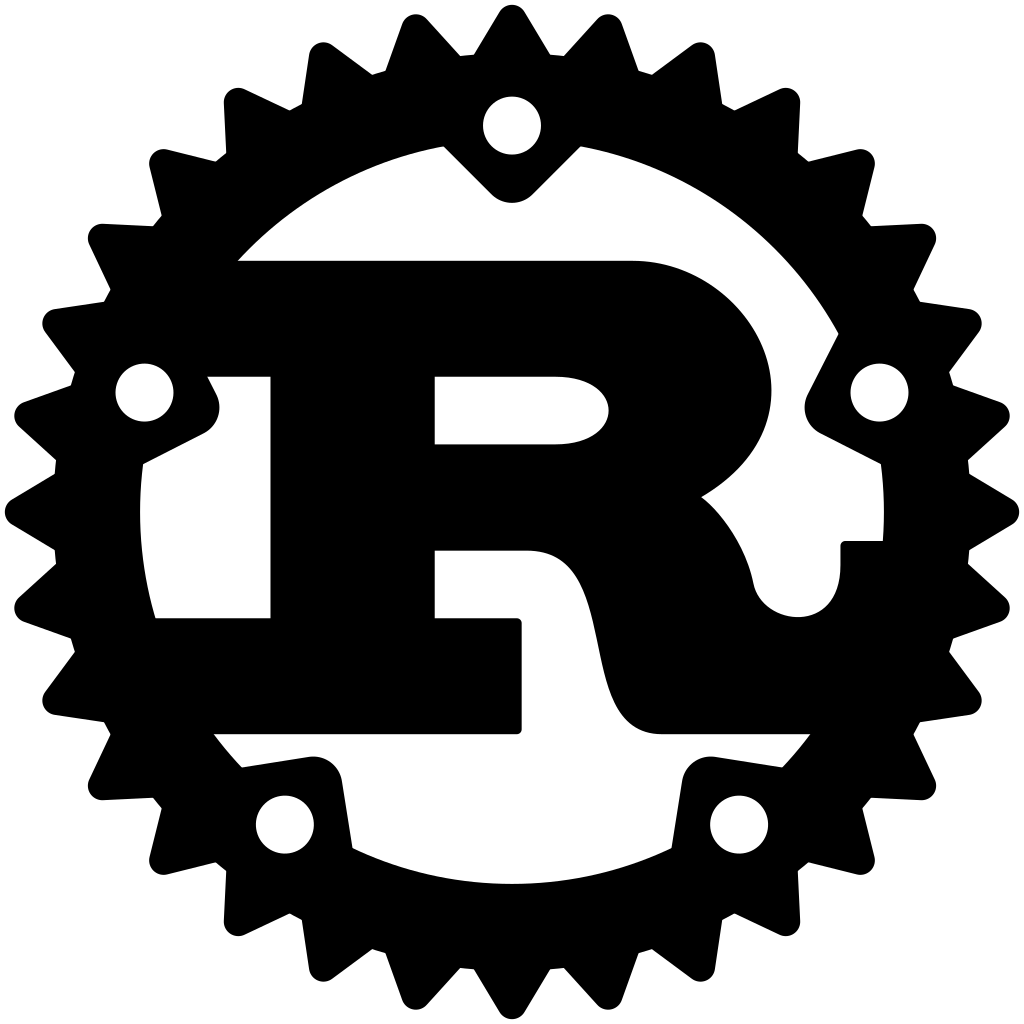
\includegraphics[width=\textwidth]{Figuras/Rust Logo.svg.png}
        \end{figure}
    \end{column}
    \end{columns}
\end{frame}

\begin{frame}{Fearless Concurrency}
    \begin{figure}
        \centering
        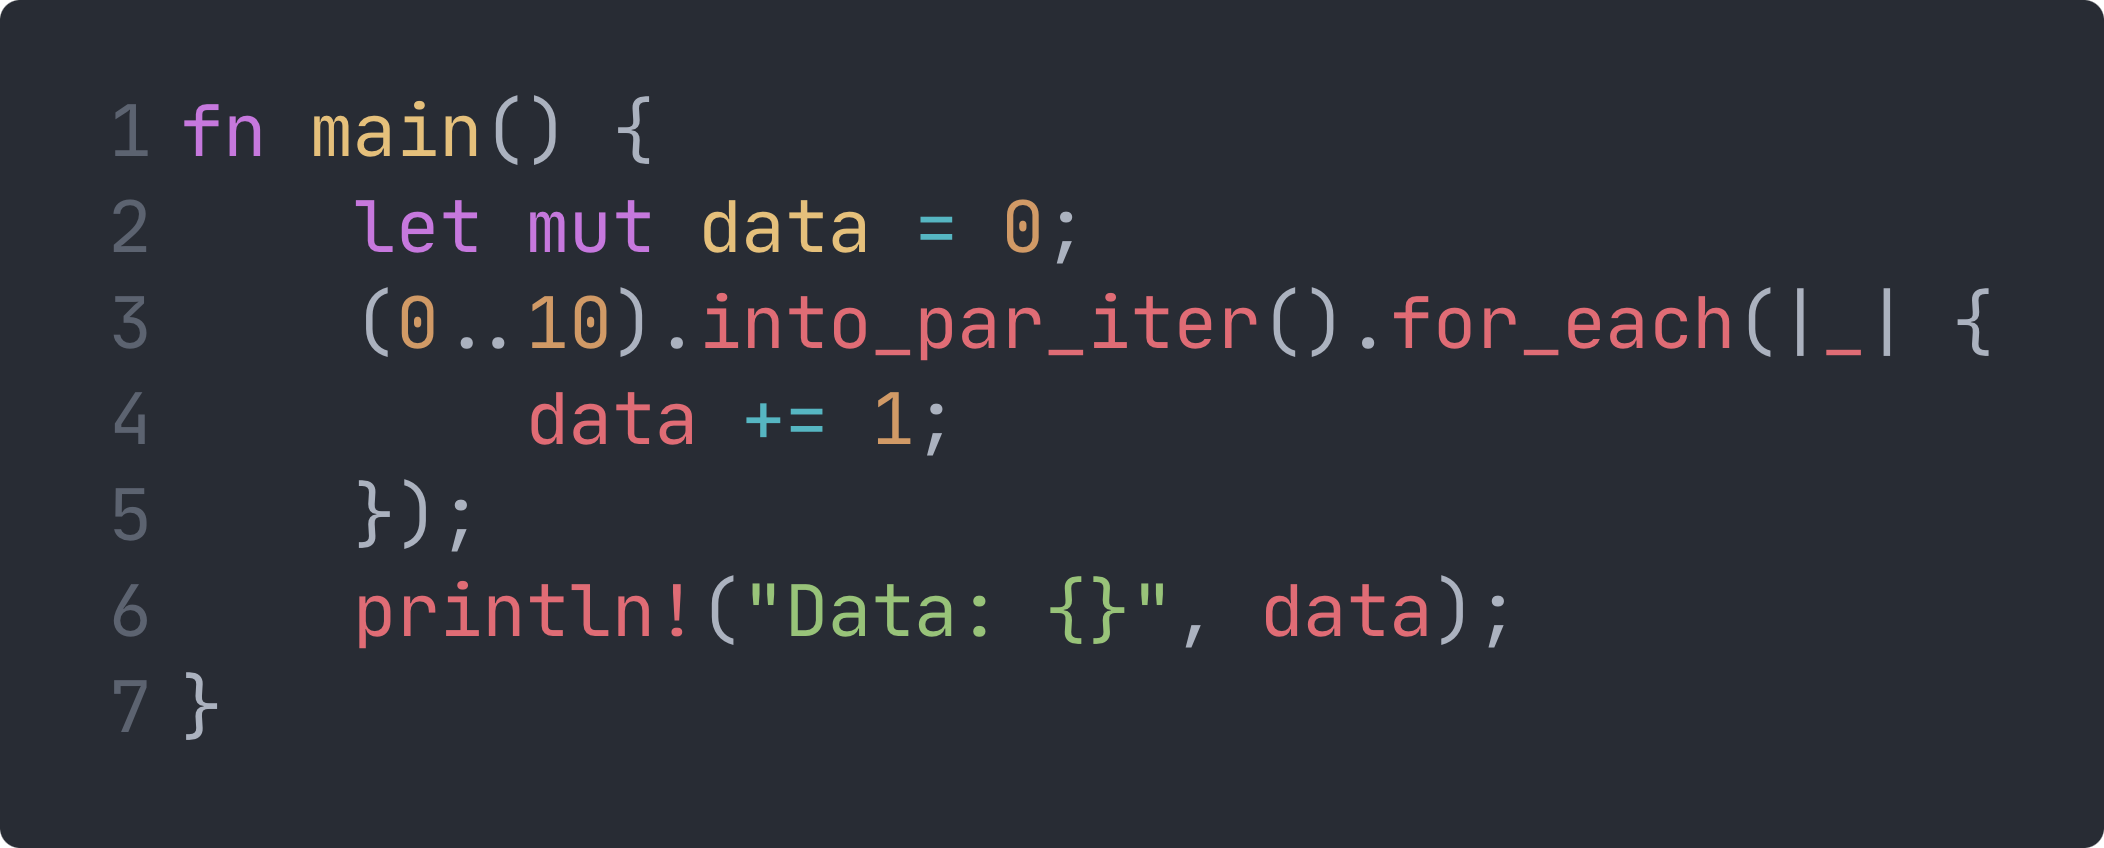
\includegraphics[width=\textwidth]{Figuras/fearlessconcurrency.png}
    \end{figure}
\end{frame}

\begin{frame}{Técnicas e Ferramentas}
    \begin{columns}
    \begin{column}{0.9\textwidth}
    C++:
    \begin{itemize}
        \item[--] Excelente suporte a \textit{GPUs}.
        \item[--] \textit{OpenAcc}.
        \item[--] Comunicação por meio de \textit{Foreign Function Interface}.
    \end{itemize}
    \end{column}

    \begin{column}{0.1\textwidth}
        \begin{figure}
            
\includegraphics[width=\textwidth]{Figuras/C++ Logo.png}
        \end{figure}
    \end{column}
    \end{columns}
\end{frame}

\begin{frame}{Cenário experimental}
    Métricas:
    \begin{itemize}
        \item[--] Speedup, Eficiência, Escalabilidade, Overhead, Utilização de recursos.
    \end{itemize}

    Base de dados aberta:
    \begin{itemize}
        \item[--] Dados reais e sintéticos.
        \item[--] Grafos de diversos tamanhos e formatos.
        \item[--] \textit{Politecnico di Milano}.
    \end{itemize}

    Infraestrutura local do LabP2D:
    \begin{itemize}
        \item[--] 2 CPUs Intel Xeon Silver 2.2GHz.
        \item[--] NVIDIA RTX 3090 24GB.
    \end{itemize}
\end{frame}

    \include{Slides/Proposta/testes}

    \section[]{Conclusões Parciais}
    \begin{frame}{Conclusões Parciais}
    \begin{itemize}
        \item Realizou-se uma revisão sobre Computação em Nuvem, Cloud-Edge Continuum , Arquiteturas Paralelas e Algoritmos Determinísticos.
        \item O trabalho apresenta um framework inovador para auxiliar no problema de escalonamento de recursos dentro do paradigma de Edge-Cloud Continuum.
    \end{itemize}
\end{frame}
    \begin{frame}{Cronograma}
    \begin{enumerate}
        \item Estudo sobre \textit{Cloud-Edge Continuum}.
        \item Estudo sobre escalonamento de tarefas em \textit{Cloud-Edge Continuum}.
        \item Estudo de técnicas de programação em arquiteturas paralelas.
        \item Seleção de algoritmos candidatos.
        \item Implementação e composição do \textit{framework}.
        \item Avaliação do \textit{framework} proposto.
        \item Redação do texto.
    \end{enumerate}
\end{frame}

\begin{frame}{Cronograma}
    \begin{table}[htpd]
        \tiny
        \centering
        \noindent \begin{tabular}{|c|c|c|c|c|c|c|c|c|c|c|c|c|}
            \hline
            \multirow{2}{*}{\textbf{\small{Etapas}}} & \multicolumn{5}{|c|}{\textbf{\small{2023/2}}} &
            \multicolumn{6}{|c|}{\textbf{\small{2024/1}}} \\
            \cline{2-12}
            &\textbf{Ago} & \textbf{Set} & \textbf{Out} & \textbf{Nov} & \textbf{Dez} & \textbf{Jan} & 
            \textbf{Fev} & \textbf{Mar} & \textbf{Abr} & \textbf{Maio} & \textbf{Jun} \\
            \hline
            \textbf{\small{1}}  & \cellcolor{gray} & \cellcolor{gray} &  &   &   &   &   &   &   &   &   \\
            \hline
            \textbf{\small{2}}  &   & \cellcolor{gray} & \cellcolor{gray} &   &   &   &   &   &   &   &   \\
            \hline
            \textbf{\small{3}}  &   & \cellcolor{gray} & \cellcolor{gray} &   &   &   &   &   &   &   &   \\
            \hline
            \textbf{\small{4}}  &   &   & \cellcolor{gray} & \cellcolor{gray} & \cellcolor{gray} &  &  &  &  &  &   \\
            \hline
            \textbf{\small{5}}  &   &   &   &   & \cellcolor{gray} & \cellcolor{gray} & \cellcolor{gray} & \cellcolor{gray} &  &  &  \\
            \hline
            \textbf{\small{6}}  &   &   &   &   &   &   & \cellcolor{gray} & \cellcolor{gray} & \cellcolor{gray} &   &   \\
            \hline
            \textbf{\small{7}}  & \cellcolor{gray} & \cellcolor{gray} & \cellcolor{gray} & \cellcolor{gray} & \cellcolor{gray} & \cellcolor{gray} & \cellcolor{gray} & \cellcolor{gray} & \cellcolor{gray} & \cellcolor{gray} & \cellcolor{gray} \\
            \hline
        \end{tabular} 
        \label{tab:Cronograma}
        \caption{Cronograma Proposto}
    \end{table}
\end{frame}

    % \section[]{Referências}
    % \begin{frame}[allowframebreaks]{Referências}
    %     \bibliography{referencias}
    % \end{frame}

\end{document}